% 59-11(인쇄 59쪽) — 가로 4칸·세로 3칸 도로망. P 는 왼쪽 아래 모퉁이, Q 는 오른쪽 위 모퉁이, A 는 P 에서 오른쪽 1칸·위 1칸인 교차점.
% 스캔 그림이 흐려 TikZ 로 다시 그림. 라벨은 원문에 있는 P·Q·A 셋뿐이고 경로 수는 적지 않는다.
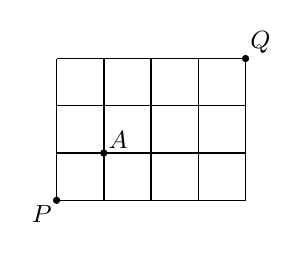
\begin{tikzpicture}[scale=0.6, line width=0.5pt]
  \draw[step=1] (0,0) grid (4,3);
  \fill (0,0) circle (2.2pt);
  \fill (4,3) circle (2.2pt);
  \fill (1,1) circle (2.2pt);
  \node[anchor=north east, inner sep=1.5pt, font=\small] at (0,0) {$\pt{P}$};
  \node[anchor=south west, inner sep=1.5pt, font=\small] at (4,3) {$\pt{Q}$};
  \node[anchor=south west, inner sep=1.5pt, font=\small] at (1,1) {$\pt{A}$};
\end{tikzpicture}
